\documentclass[11pt,spanish]{article} % Tipo y tamaño de letra del documento.


\usepackage[utf8]{inputenc}
\usepackage{subfiles}
\usepackage{biblatex}
\addbibresource{references.bib}
\usepackage{multicol}
\usepackage{amsfonts}
\usepackage{blindtext}
\usepackage{mathrsfs}
\usepackage{amsmath}
\usepackage{siunitx}
\usepackage{centernot}
\usepackage[shortlabels]{enumitem}
\usepackage{subfig}
\usepackage{datetime}
\usepackage{listingsutf8}
\usepackage[spanish]{babel}
\usepackage{tikz}
\usepackage{hyperref}
\usepackage[vlined,ruled,linesnumbered]{algorithm2e}
\usepackage{listings}
\usepackage{float}
\usepackage{url}
\usepackage{csquotes}
\usepackage{fourier} %font
\usepackage[top=2cm, bottom=2cm, left=2.5cm, right=2.5cm]{geometry}
\usepackage{pgfplots}
\usepackage{fancyhdr}
\usepackage{mdframed}
\usepackage{tikzducks}
\usepackage[nameinlink]{cleveref}
\usepackage{epigraph} 

\pgfplotsset{compat=1.18}

\usetikzlibrary{shapes.arrows, shapes.geometric, arrows.meta,angles,quotes,positioning,arrows,fit,quotes,calc}
\tikzset{>=latex} 

\setlength\algomargin{1em} 
\SetFuncSty{sc} 
\SetCommentSty{em} 


\Crefname{figure}{Fig.}{Figs.}
\newcommand\crefrangeconjunction{--}
\Crefname{table}{Tabla}{Tablas}
\Crefname{subsubsection}{Subsubsec.}{Subsubsections}
\Crefname{subsection}{Subsec.}{Subsections}
\Crefname{section}{Sec.}{Sections}
\Crefname{equation}{eq.}{eqs.}
\crefname{thm}{Theorem}{theorems}
\Crefname{thm}{Theorem}{Theorems} 

\definecolor{algoco}{rgb}{0,0.4,1}

\hypersetup{
  colorlinks=true,
  linkcolor=algoco,
  citecolor=blue,
  urlcolor=blue,
}

\lstset{
extendedchars=true
inputencoding=utf8/latin1,
basicstyle=\footnotesize\sffamily\color{black},
commentstyle=\slshape \color{gray},
numbers=left,
numbersep=10pt,
numberstyle=\tiny\color{red!80!black},
keywordstyle=\color{red!80!magenta},
showspaces=false,
showstringspaces=false,
stringstyle=\color{cyan!80!black},
tabsize=2,
literate={á}{{\'a}}1 {é}{{\'e}}1 {í}{{\'i}}1 {ó}{{\'o}}1 {ú}{{\'u}}1,
frame = single, 
numbers = none,
float, floatplacement = ht, captionpos = b,
xleftmargin = 2em, xrightmargin = 2em, 
}

\newcommand{\ub}[1]{\underbrace{#1}}
\newcommand\tcm{\textcolor{magenta}}
\newcommand\tca{\textcolor{algoco}}

\setlength\epigraphwidth{.7\textwidth} 

\newcommand{\tnum}{2 y 3} % reemplace 2 por el número de la tarea
\newcommand{\sem}{2024-2} % reemplace 2024-2 por el semestre correspondiente
\newcommand{\campus}{San Joaquín \\ Santiago} % reemplace Casa Central por el campus correspondiente
\newcommand{\rolusm}{202273545-7} % reemplace 2025073100-1 por su rol
\newcommand{\namestudent}{Joaquín Domínguez Bustos} % reemplace Al Goritmo Pérez por su nombre

\headheight=14pt
\linespread{1.3}
\author{\namestudent}
\pagestyle{fancy}
\fancyhf{}%
\fancyfoot[R]{ \namestudent \\ \rolusm}
\fancyfoot[L]{Campus \campus} 
\fancyfoot[C]{\thepage}
\rhead{2024-2}
\lhead{INF-221}
\renewcommand{\headrulewidth}{0.4pt}
\renewcommand{\footrulewidth}{0.4pt}
\newbool{programs}
\boolfalse{programs}
\chead{REPORTE TAREA \tnum~}



\title{
  \huge
  \textbf{REPORTE TAREA \tnum~ \\ ALGORITMOS Y COMPLEJIDAD} \\[1ex]
  \emph{\textquote{Explorando la Distancia entre Cadenas, una Operación a la Vez}}
  }

  
\date{
  \small
  \today\\
  \currenttime
}




\begin{document}
\maketitle
\thispagestyle{fancy} 
\vspace{-1.0\baselineskip}




\begin{abstract}
  \textit{ 
    Este informe aborda el problema de la distancia de Damerau-Levenshtein mediante dos enfoques principales: 
algoritmos de fuerza bruta y programación dinámica. Se analiza cómo los costos asociados a operaciones como eliminación,
inserción, reemplazo y transposición afectan la complejidad temporal de las soluciones propuestas. El trabajo incluye un diseño 
detallado de los algoritmos, su implementación en código y la evaluación experimental en diversos conjuntos de datos. Los resultados 
muestran una clara ventaja en eficiencia para la programación dinámica, aunque a costa de un mayor uso de memoria, mientras que la 
fuerza bruta puede ser útil en casos específicos con cadenas vacías.


  }
     
\end{abstract}

\setcounter{tocdepth}{1}
\tableofcontents


\newpage
\section{Introducción}
En el ámbito de las Ciencias de la Computación, el análisis y diseño de algoritmos constituye un área fundamental, ya que establece las bases para resolver problemas complejos de manera eficiente. Uno de los problemas clásicos en este campo es la comparación de cadenas, esencial en aplicaciones como la corrección ortográfica, el reconocimiento de patrones y la bioinformática. La distancia de Damerau-Levenshtein, que mide el costo mínimo para transformar una cadena en otra mediante operaciones de inserción, eliminación, reemplazo y transposición, proporciona una métrica versátil y ampliamente utilizada.

A pesar de su relevancia, este problema plantea desafíos significativos en términos de eficiencia computacional, especialmente cuando se utilizan algoritmos de alta complejidad como la fuerza bruta. Las soluciones modernas, como las basadas en programación dinámica, prometen una mejora considerable, aunque con un costo adicional de memoria. Sin embargo, existe una brecha en la comprensión detallada del impacto de las operaciones individuales y los escenarios específicos sobre el rendimiento de estos algoritmos.

El propósito de este informe es estudiar y comparar ambos enfoques, fuerza bruta y programación dinámica, en el contexto del cálculo de la distancia de Damerau-Levenshtein. A través de un diseño detallado, implementaciones prácticas y experimentos controlados, se busca determinar cómo los costos asociados a cada operación afectan la complejidad temporal y espacial de las soluciones. Además, se evalúan casos particulares, como cadenas vacías o con caracteres repetidos, para identificar patrones de rendimiento y posibles áreas de optimización.




\newpage
\section{Diseño y Análisis de Algoritmos} 
\begin{mdframed}
    \textbf{La extensión máxima para esta sección es de 5 páginas.}
\end{mdframed}

Diseñar un algoritmo por cada técnica de diseño de algoritmos mencionada en la sección de objetivos. Cada algoritmo debe resolver el problema de distancia mínima de edición extendida, dadas dos cadenas \texttt{S1} y \texttt{S2}, utilizando las operaciones y costos especificados.

\begin{itemize}
    \item Describir la solución diseñada. 
    \item Incluir pseudocódigo (ver ejemplo \cref{alg:mi_algoritmo_1})
    \item Proporciones un ejemplo paso a paso de la ejecución de sus algoritmos que ilustren cómo sus algoritmos manejan diferentes escenarios, particularmente donde las
    transposiciones o los costos variables afectan el
    resultado. Haga referencias a los programas expresados en psudocódigo (además puede hacer diagramas).
    \item Analizar la Complejidad temporal y espacial de los algoritmos diseñados en términos de las longitudes de las cadenas de entrada $S1$ y $S2$
    \item Discute cómo la inclusión de transposiciones y costos   variables impacta la complejidad.
\end{itemize}

Los pseudocódigos los he diseñado utilizando el paquete \citetitle{algorithm2e} \cite{algorithm2e} para la presentación de algoritmos. Se recomienda consultar \citetitle{ctan-algorithm2e} \cite{ctan-algorithm2e} y \citetitle{overleaf-algorithms} \cite{overleaf-algorithms}.

Todo lo correspondiente a esta sección es, digamos, en ``\href{https://dle.rae.es/metáfora}{lapiz y papel}'', en el sentido de que no necesita de implementaciones ni resultados experimentales. 

\begin{mdframed}
    Recuerde que lo importante es diseñar algoritmos que cumplan con los paradigmas especificados. 
\end{mdframed}

\begin{mdframed}
    Si se utiliza algún código, idea, o contenido extraído de otra fuente, este \textbf{debe} ser citado en el lugar exacto donde se utilice, en lugar de mencionarlo al final del informe. 
\end{mdframed}



\subsection{Fuerza Bruta}

%\epigraph{\textit{``Indeed, brute force is a perfectly good technique in many cases; the real question is, can we use brute force in such a way that we avoid the worst-case behavior?''}}{--- \citeauthor{taocv3}, \citeyear{taocv3} \cite{taocv3}}

\begin{algorithm}[H]
    \SetKwProg{myproc}{Procedure}{}{end}
    \SetKwFunction{BF}{BF}  % Nombre de la función principal
    \SetKwFunction{CostoIns}{costo\_ins}  % Función de costo de inserción
    \SetKwFunction{CostoDel}{costo\_del}  % Función de costo de eliminación
    \SetKwFunction{CostoSub}{costo\_sub}  % Función de costo de sustitución
    \SetKwFunction{CostoTrans}{costo\_trans}  % Función de costo de transposición

    \DontPrintSemicolon
    \footnotesize

    % Definición del algoritmo principal
    \myproc{\BF{S1, S2, i, j}}{
        \uIf{$i \geq \text{longitud}(S1)$ \textbf{and} $j \geq \text{longitud}(S2)$}{
            \Return $0$\;
        }
        
        \uIf{$i \geq \text{longitud}(S1)$}{
            \Return $\CostoIns{S2[j]} + \BF{S1, S2, i, j+1}$\;
        }
        
        \uIf{$j \geq \text{longitud}(S2)$}{
            \Return $\CostoDel{S1[i]} + \BF{S1, S2, i+1, j}$\;
        }
        
        $elim \gets \CostoDel{S1[i]} + \BF{S1, S2, i+1, j}$\;
        $ins \gets \CostoIns{S2[j]} + \BF{S1, S2, i, j+1}$\;
        $remp \gets \CostoSub{S1[i], S2[j]} + \BF{S1, S2, i+1, j+1}$\;
        $transp \gets \infty$\;
        
        \If{$i+1 < \text{longitud}(S1)$ \textbf{and} $j+1 < \text{longitud}(S2)$ \textbf{and} $S1[i] = S2[j+1]$ \textbf{and} $S1[i+1] = S2[j]$}{
            $transp \gets \CostoTrans{S1[i], S1[i+1]} + \BF{S1, S2, i+2, j+2}$\;
        }
        
        \Return $\min(\{elim, ins, remp, transp\})$\;
    }
    \caption{Algoritmo de Fuerza Bruta para la Transformación de Cadenas}
    \label{alg:mi_algoritmo_1}
\end{algorithm}


\subsubsection{Ejemplo de ejecución}

Consideremos las cadenas de longitud 3:  
\[
S_1 = \texttt{abc}, \quad S_2 = \texttt{adc}.
\]

Supongamos que los costos de las operaciones son:
\begin{itemize}
    \item \( \text{costo\_ins}(x) = 1 \)
    \item \( \text{costo\_del}(x) = 1 \)
    \item \( \text{costo\_sub}(x, y) = 1 \) si \( x \neq y \), \( 0 \) en caso contrario
    \item \( \text{costo\_trans}(x, y) = 1 \)
\end{itemize}

\subsection*{Paso a Paso de la Ejecución}

\begin{enumerate}
    \item Llamada inicial: \( BF(\texttt{abc}, \texttt{adc}, 0, 0) \).
    \begin{itemize}
        \item \( S_1[0] = \texttt{a}, S_2[0] = \texttt{a} \). Como son iguales, el algoritmo calcula:  
        \( \text{remp} = 0 + BF(1, 1) \).
        \item También calcula:  
        \( \text{elim} = 1 + BF(1, 0) \) y \( \text{ins} = 1 + BF(0, 1) \), mientras que no aplica transposición.
    \end{itemize}

    \item Segunda llamada: \( BF(\texttt{abc}, \texttt{adc}, 1, 1) \).
    \begin{itemize}
        \item \( S_1[1] = \texttt{b}, S_2[1] = \texttt{d} \). Como son diferentes, el algoritmo calcula:  
        \( \text{remp} = 1 + BF(2, 2) \).
        \item También calcula:  
        \( \text{elim} = 1 + BF(2, 1) \),  
        \( \text{ins} = 1 + BF(1, 2) \), mientras que no aplica transposición.
    \end{itemize}

    \item Tercera llamada: \( BF(\texttt{abc}, \texttt{adc}, 2, 2) \).
    \begin{itemize}
        \item \( S_1[2] = \texttt{c}, S_2[2] = \texttt{c} \). Como son iguales, calcula:  
        \( \text{remp} = 0 + BF(3, 3) \).
        \item También calcula:  
        \( \text{elim} = 1 + BF(3, 2) \) y \( \text{ins} = 1 + BF(2, 3) \), mientras que no aplica transposición.
    \end{itemize}

    \item Llamada base: \( BF(\texttt{abc}, \texttt{adc}, 3, 3) \).
    \begin{itemize}
        \item Caso base: retorna 0 porque ambas cadenas han sido procesadas completamente.
    \end{itemize}
\end{enumerate}

\subsection*{Resultado}

El costo mínimo para transformar \( S_1 \) en \( S_2 \) es \( 1 \). La única operación necesaria es reemplazar \( \texttt{b} \) por \( \texttt{d} \).

\subsubsection{Análisis de complejidad espacial y temporal}

    En cada llamada que se realiza se pueden generar hasta 4 subproblemas nuevos, así tambien es necesario recorrer cada cadena hasta el final de la misma mediante 
    el uso de los indices $(i,j)$, los cuales llegaran a un valor final $(n,m)$ en donde $n$ y $m$ son los largos de $S1$ y $S2$ respectivamente, por lo que el 
    número total de operaciones será aproximadamente $4^{\min(n,m)}$, dando así que la complejidad temporal pertence a $O(4^{\min(n,m)})$. Por otra parte,
    la complejidad espacial asociada a esta implementacion sería $O(1)$ puesto que no se utiliza ninguna estructura de datos adicional al tamaño de la entrada y
    para las llamadas recursivas se apoya en el stack.


\subsection{Programación Dinámica}

\epigraph{\textit{Dynamic programming is not about filling in tables. It's about smart recursion!}}{\citeauthor{algorithms_erickson}, \citeyear{algorithms_erickson} \cite{algorithms_erickson}}

\begin{enumerate}[1)]
    \item Describa la solución recursiva.
    \item Escriba la relación de recurrencia, incluyendo condiciones y casos base.
    \item Identifique subproblemas.
    \item Defina estructura de datos a utilizar y especifique el orden de calculo que realiza su programa que utiliza programación dinámica. 
\end{enumerate}

\subsubsection{Descripción de la solución recursiva}

\subsubsection{Relación de recurrencia}

\subsubsection{Identificación de subproblemas}

\subsubsection{Estructura de datos y orden de cálculo}

\subsubsection{Algoritmo utilizando programación dinámica}



\begin{algorithm}[H]

    \SetKwProg{myproc}{Procedure}{}{}
    \SetKwFunction{AlgorithmName}{AlgorithmName}  % Cambia 'AlgorithmName' por el nombre del enfoque elegido
    \SetKwFunction{AuxiliaryFunction}{AuxiliaryFunction}  % Función auxiliar de ejemplo
    
    \DontPrintSemicolon
    \footnotesize

    % Definición del algoritmo principal
    \myproc{\AlgorithmName{S1, S2}}{
    \uIf{S1 está vacía}{
        \Return longitud de S2\;  % Return explícito si S1 está vacía
    }
    \uElseIf{S2 está vacía}{
        \Return longitud de S1\;  % Return explícito si S2 está vacía
    }
    \uElseIf{S1[0] = S2[0]}{
        \Return \AlgorithmName{S1[1:], S2[1:]}  % Llamada recursiva
    }
    \Else{
        % Ejemplo de llamado a una función auxiliar
        $costo \leftarrow \AuxiliaryFunction{S1, S2}$\;
        \Return costo\;  % Retornar el valor calculado
    }
    }

    % Definición de la función auxiliar
    \myproc{\AuxiliaryFunction{S1, S2}}{
    % Acciones o cálculos auxiliares
    \uIf{S1 y S2 son similares}{
        \Return algún valor o costo\;  % Retornar el valor calculado por la función auxiliar
    }
    \Else{
        % Llamar de nuevo a la función principal
        \Return \AlgorithmName{S1 modificado, S2}\;  % Llamada recursiva y retorno del resultado
    }
    }
    \caption{Este es solo un ejemplo de cómo estructurar el pseudocódigo, con retornos explícitos y llamados a funciones.}
    \label{alg:mi_algoritmo_2}
\end{algorithm}
\newpage
\section{Implementaciones}
\begin{mdframed}
    \textbf{La extensión máxima para esta sección es de 1 página.}
\end{mdframed}

Aquí deben explicar la estructura de sus programas haciendo referencias a los archivos y funciones de su entrega. No adjunte código en esta sección.
\begin{mdframed}
    Si se utiliza algún código, idea, o contenido extraído de otra fuente, este \textbf{debe} ser citado en el lugar exacto donde se utilice, en lugar de mencionarlo al final del informe.
\end{mdframed}

\newpage
\section{Experimentos}
%\epigraph{``\textit{Non-reproducible single occurrences are of no significance to
%science.}''}{---\citeauthor{popper2005logic},\citeyear{popper2005logic} \cite{popper2005logic}}
Todos los experimentos se desarrollaron en el siguiente ambiente computacional:

\begin{itemize}
    \item \textbf{Hardware}
    \begin{itemize}
        \item \textbf{Procesador:} AMD Ryzen 5 4600H 3.0GHz
        \item \textbf{RAM:} 16GB Dual Channel 3200 MT/s DDR4 SODIMM
        \item \textbf{Almacenamiento:} 500GB SSD NVMe
    \end{itemize}
    \item \textbf{Software}
    \begin{itemize}
        \item \textbf{SO:} Windows 11 v10.0.22631.4460
        \item \textbf{Entorno:} WSL v2.3.26.0 con Ubuntu 14.2.0 y g++ 14.2.0
        \item \textbf{Python:} v3.12.3 con liberías pandas, matplotlib.pyplot, numpy, pathlib, random.
    \end{itemize}
    \item \textbf{Consideraciones}
    \begin{itemize}
        \item Se utilizó el siguiente comando para la compilacion: g++ -O3 (.cpp) -o (ejecutable).
        \item Los datasets fueron ingresados mediante entrada estandar.
        \item Los archivos de resultados finales que se utilizaron para la creacion de los graficos son una recopilacion manual de los archivos generados 
        por los algoritmos.
    \end{itemize}
\end{itemize}
\subsection{Dataset (casos de prueba)}
\begin{mdframed}
    \textbf{La extensión máxima para esta sección es de 2 páginas.}
\end{mdframed}
Es importante generar varias muestras con características similares para una misma entrada, por ejemplo, variando tamaño del input dentro de lo que les permita la infraestructura utilizada en ests informe, con el fin de capturar una mayor diversidad de casos y obtener un análisis más completo del rendimiento de los algoritmos.

\begin{mdframed}
    Aunque la implementación de los algoritmos debe ser realizada en C++, se recomienda aprovechar otros lenguajes como Python para automatizar la generación de casos de prueba, ya que es más amigable para crear gráficos y realizar análisis de los resultados. Python, con sus bibliotecas como \texttt{matplotlib} o \texttt{pandas}, facilita la visualización de los datos obtenidos de las ejecuciones de los distintos algoritmo bajo diferentes escenarios.
\end{mdframed}    

\begin{mdframed}    
    Debido a la naturaleza de las pruebas en un entorno computacional, los tiempos de ejecución pueden variar significativamente dependiendo de factores externos, como la carga del sistema en el momento de la ejecución. Por lo tanto, para obtener una medida más representativa, siempre es recomendable ejecutar múltiples pruebas con las mismas características de entrada y calcular el promedio de los resultados.
\end{mdframed}

\subsection{Resultados}

A continuacion se discuten los resultados obtenidos por cada dataset
\begin{figure}[H]
    \centering
        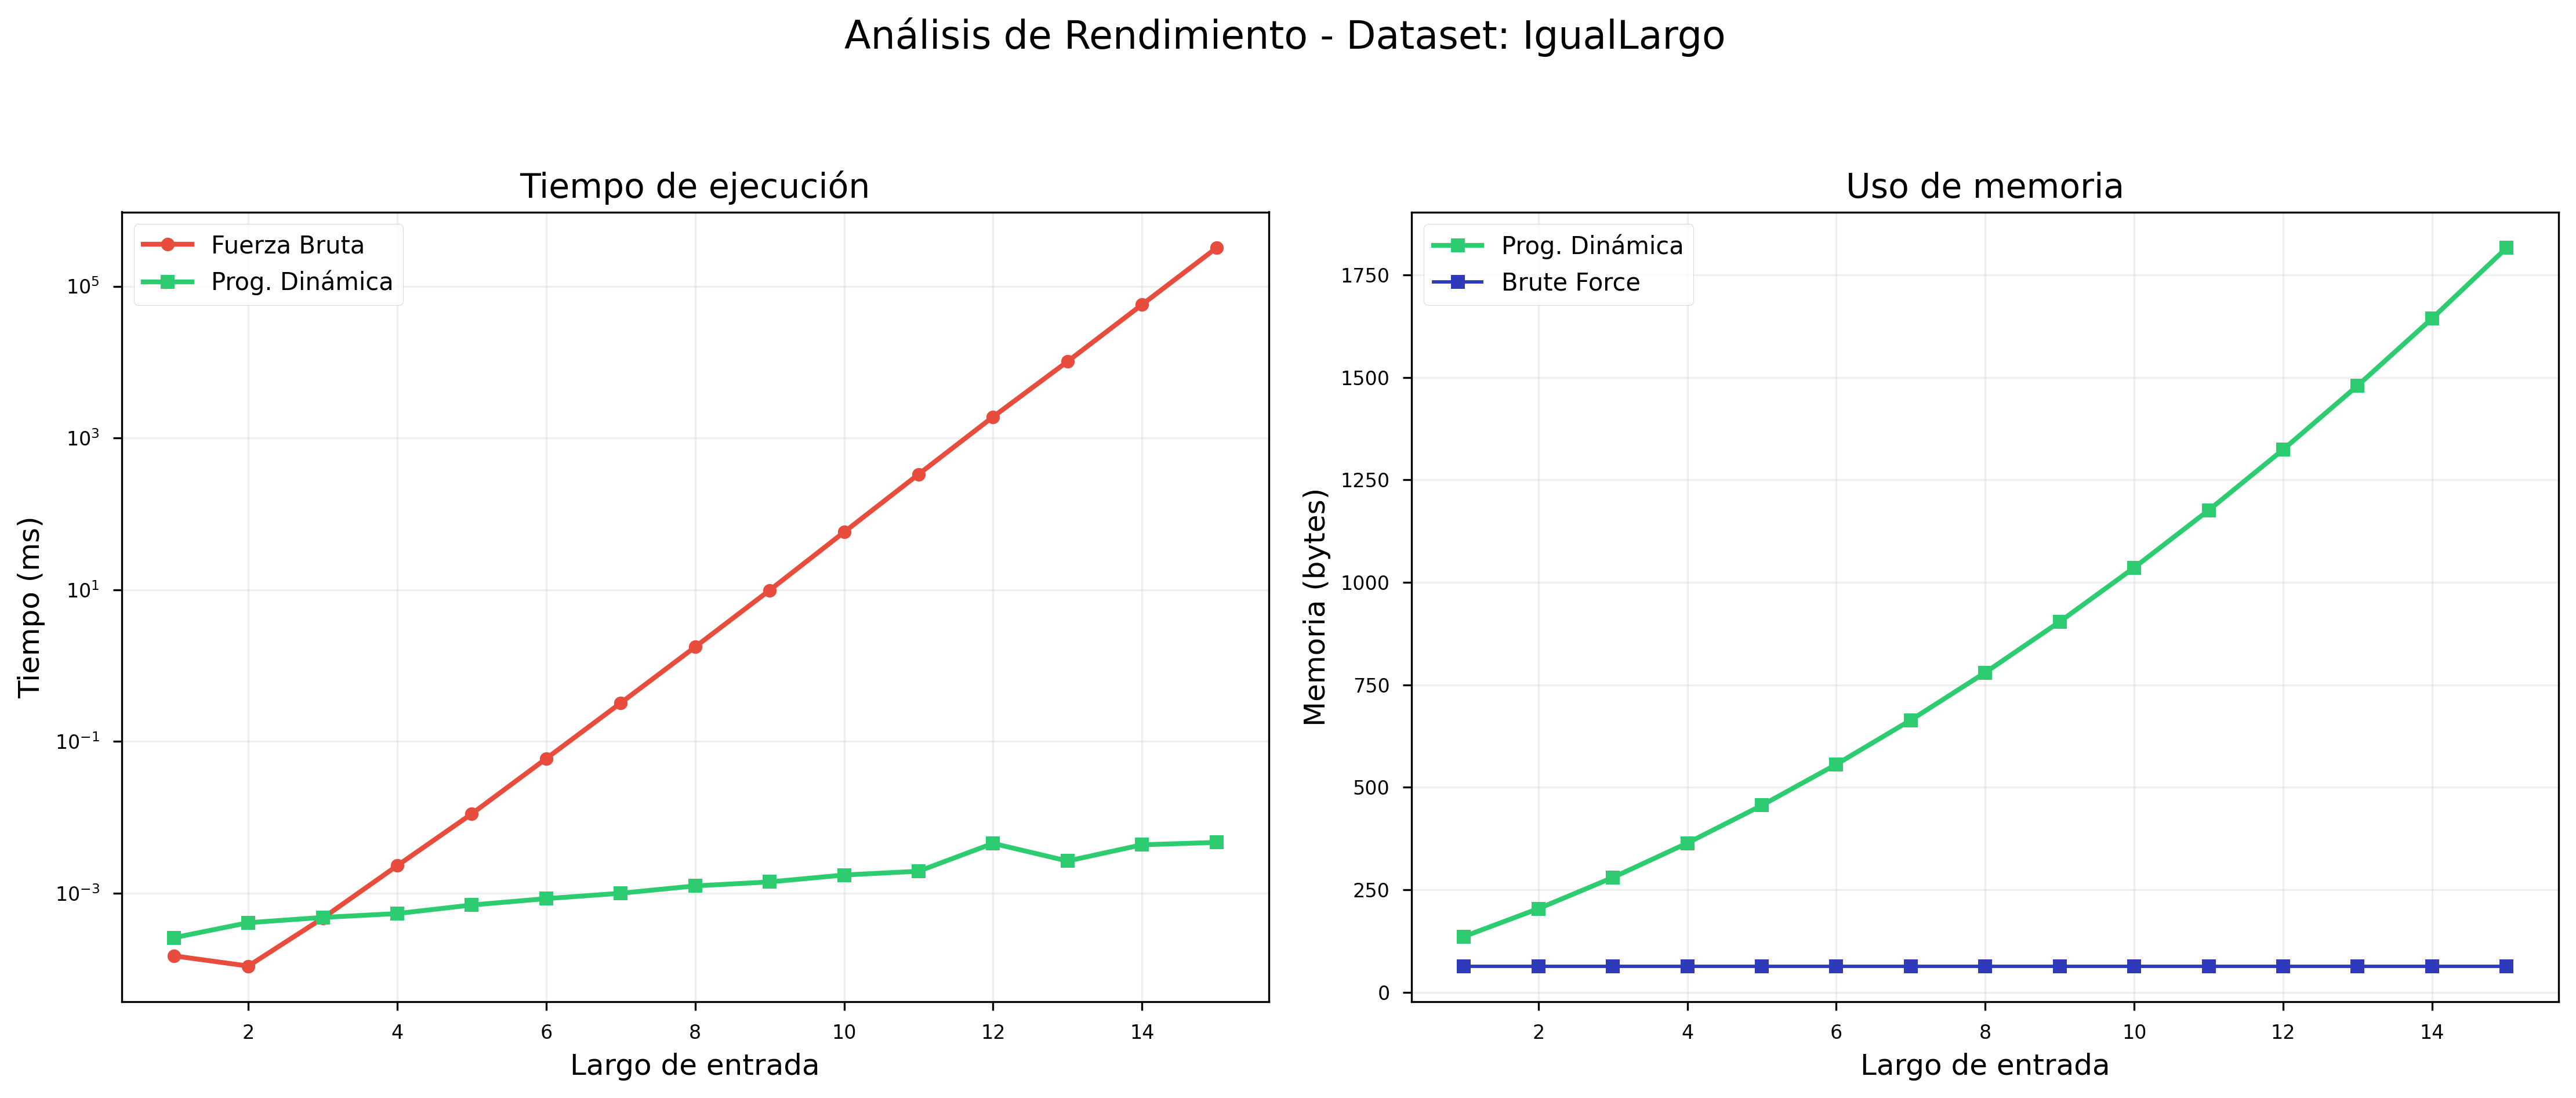
\includegraphics[width=\textwidth]{images/IgualLargo_analisis.png}
    \caption{Cadenas aleatorias de largo creciente}
    \label{fig:scatterplot_1}
\end{figure}
En el grafico de la iquierda se puede observar la inmensa diferencia en tiempo de ejecucion de ambos algoritmos a medida que el tamaño de la entrada crece,
aunque la menor complejidad temporal que maneja programacion dinamica requiere una mayor complejidad espacial.

\begin{figure}[H]
    \centering
        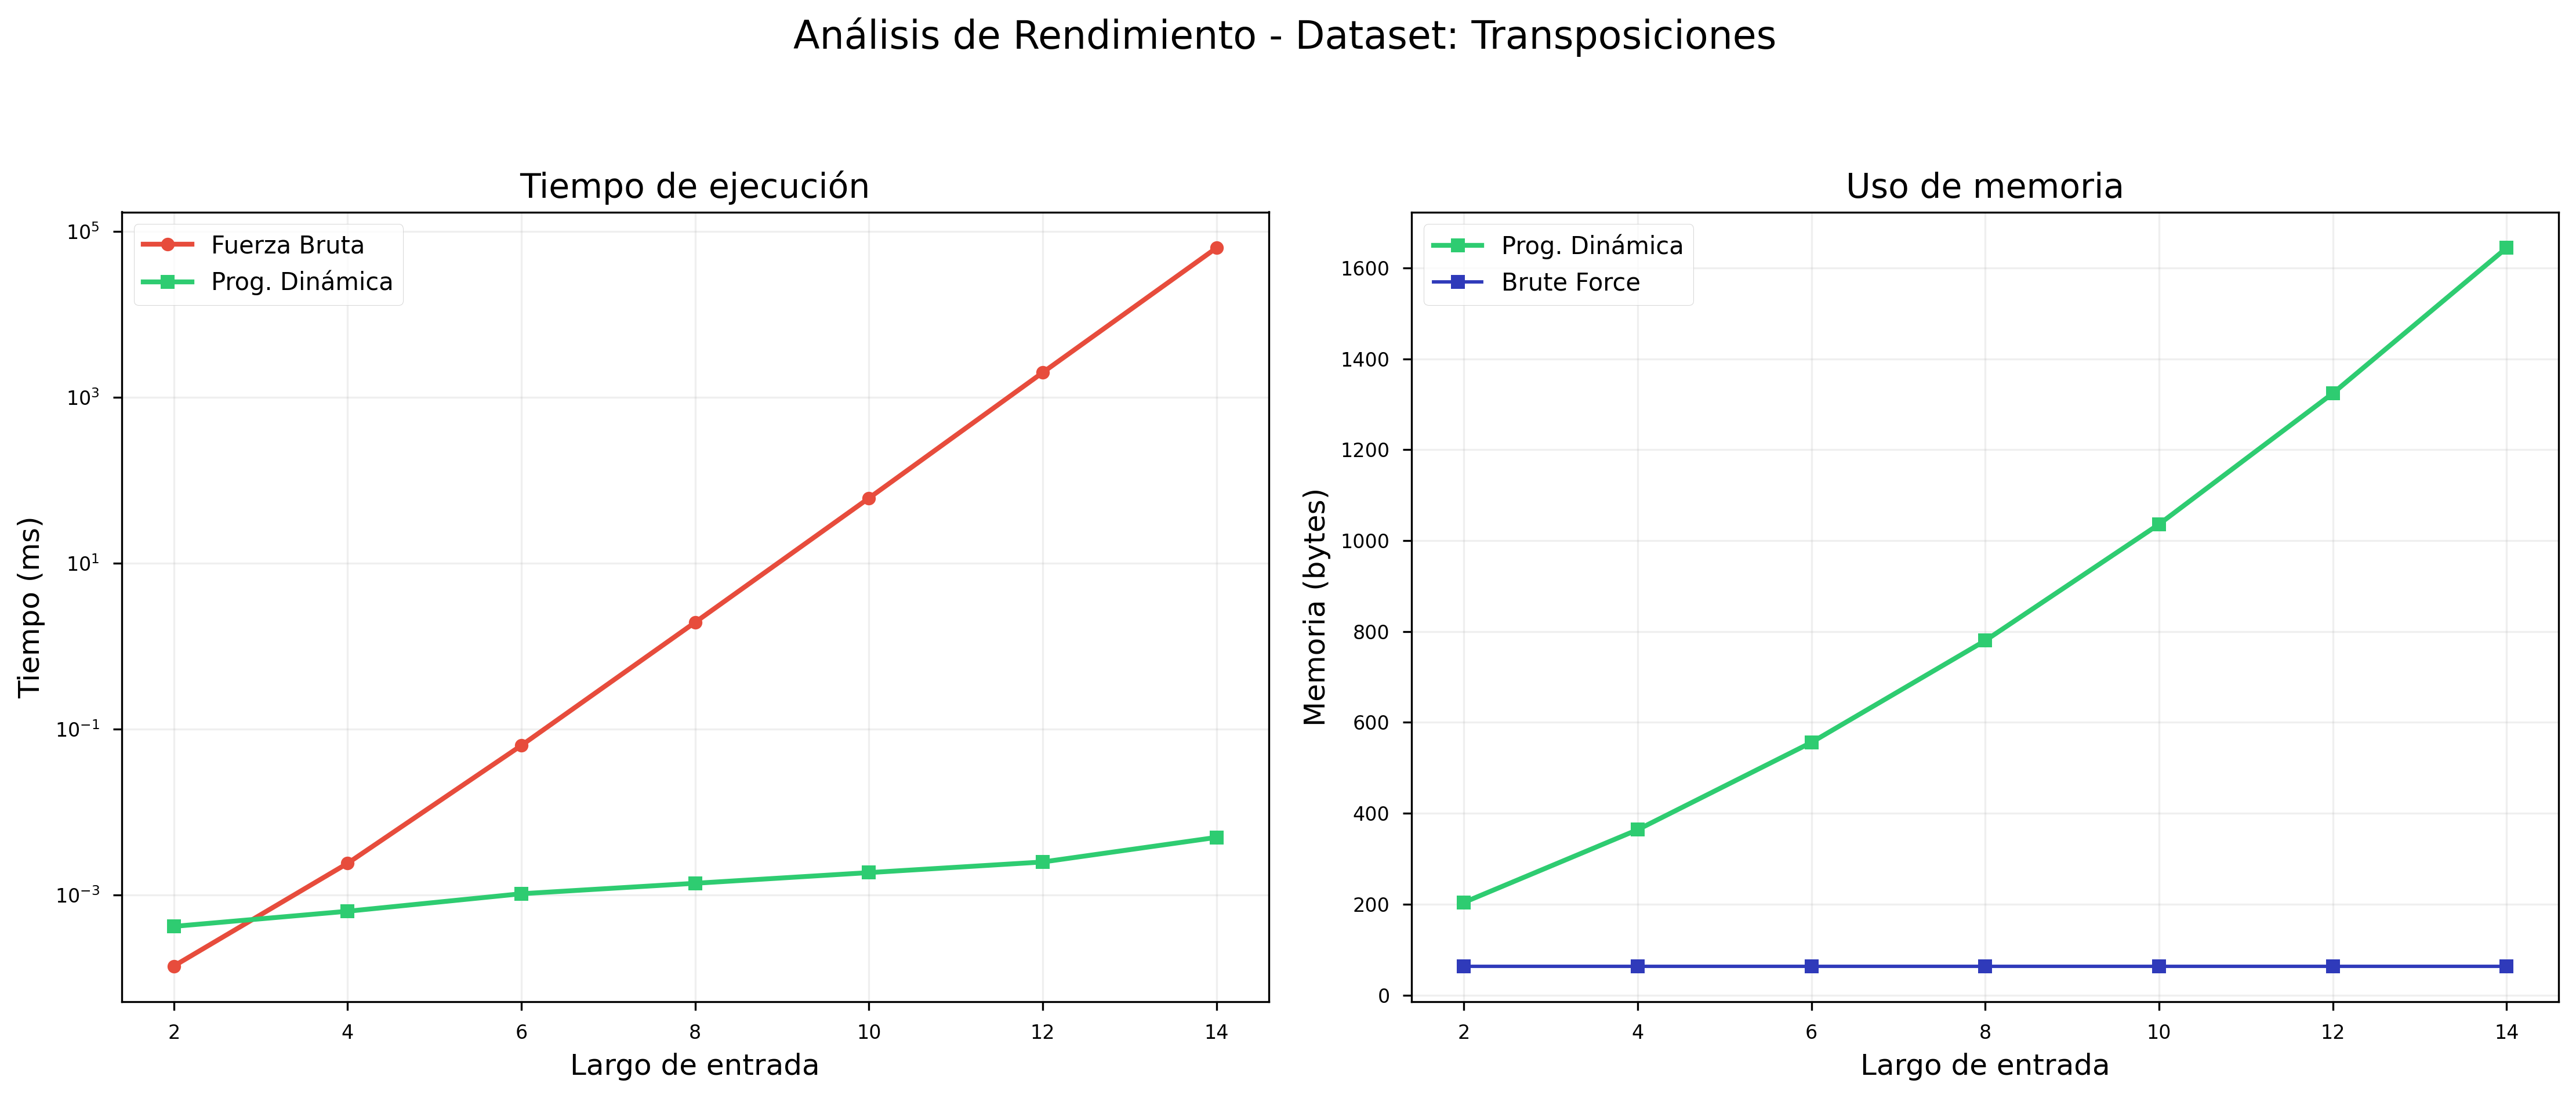
\includegraphics[width=\textwidth]{images/Transposiciones_analisis.png}
    \caption{Cadenas de pares transpuestos}
    \label{fig:scatterplot_2}
\end{figure}
\begin{figure}[H]
    \centering
    \begin{minipage}[t]{0.5\textwidth}
        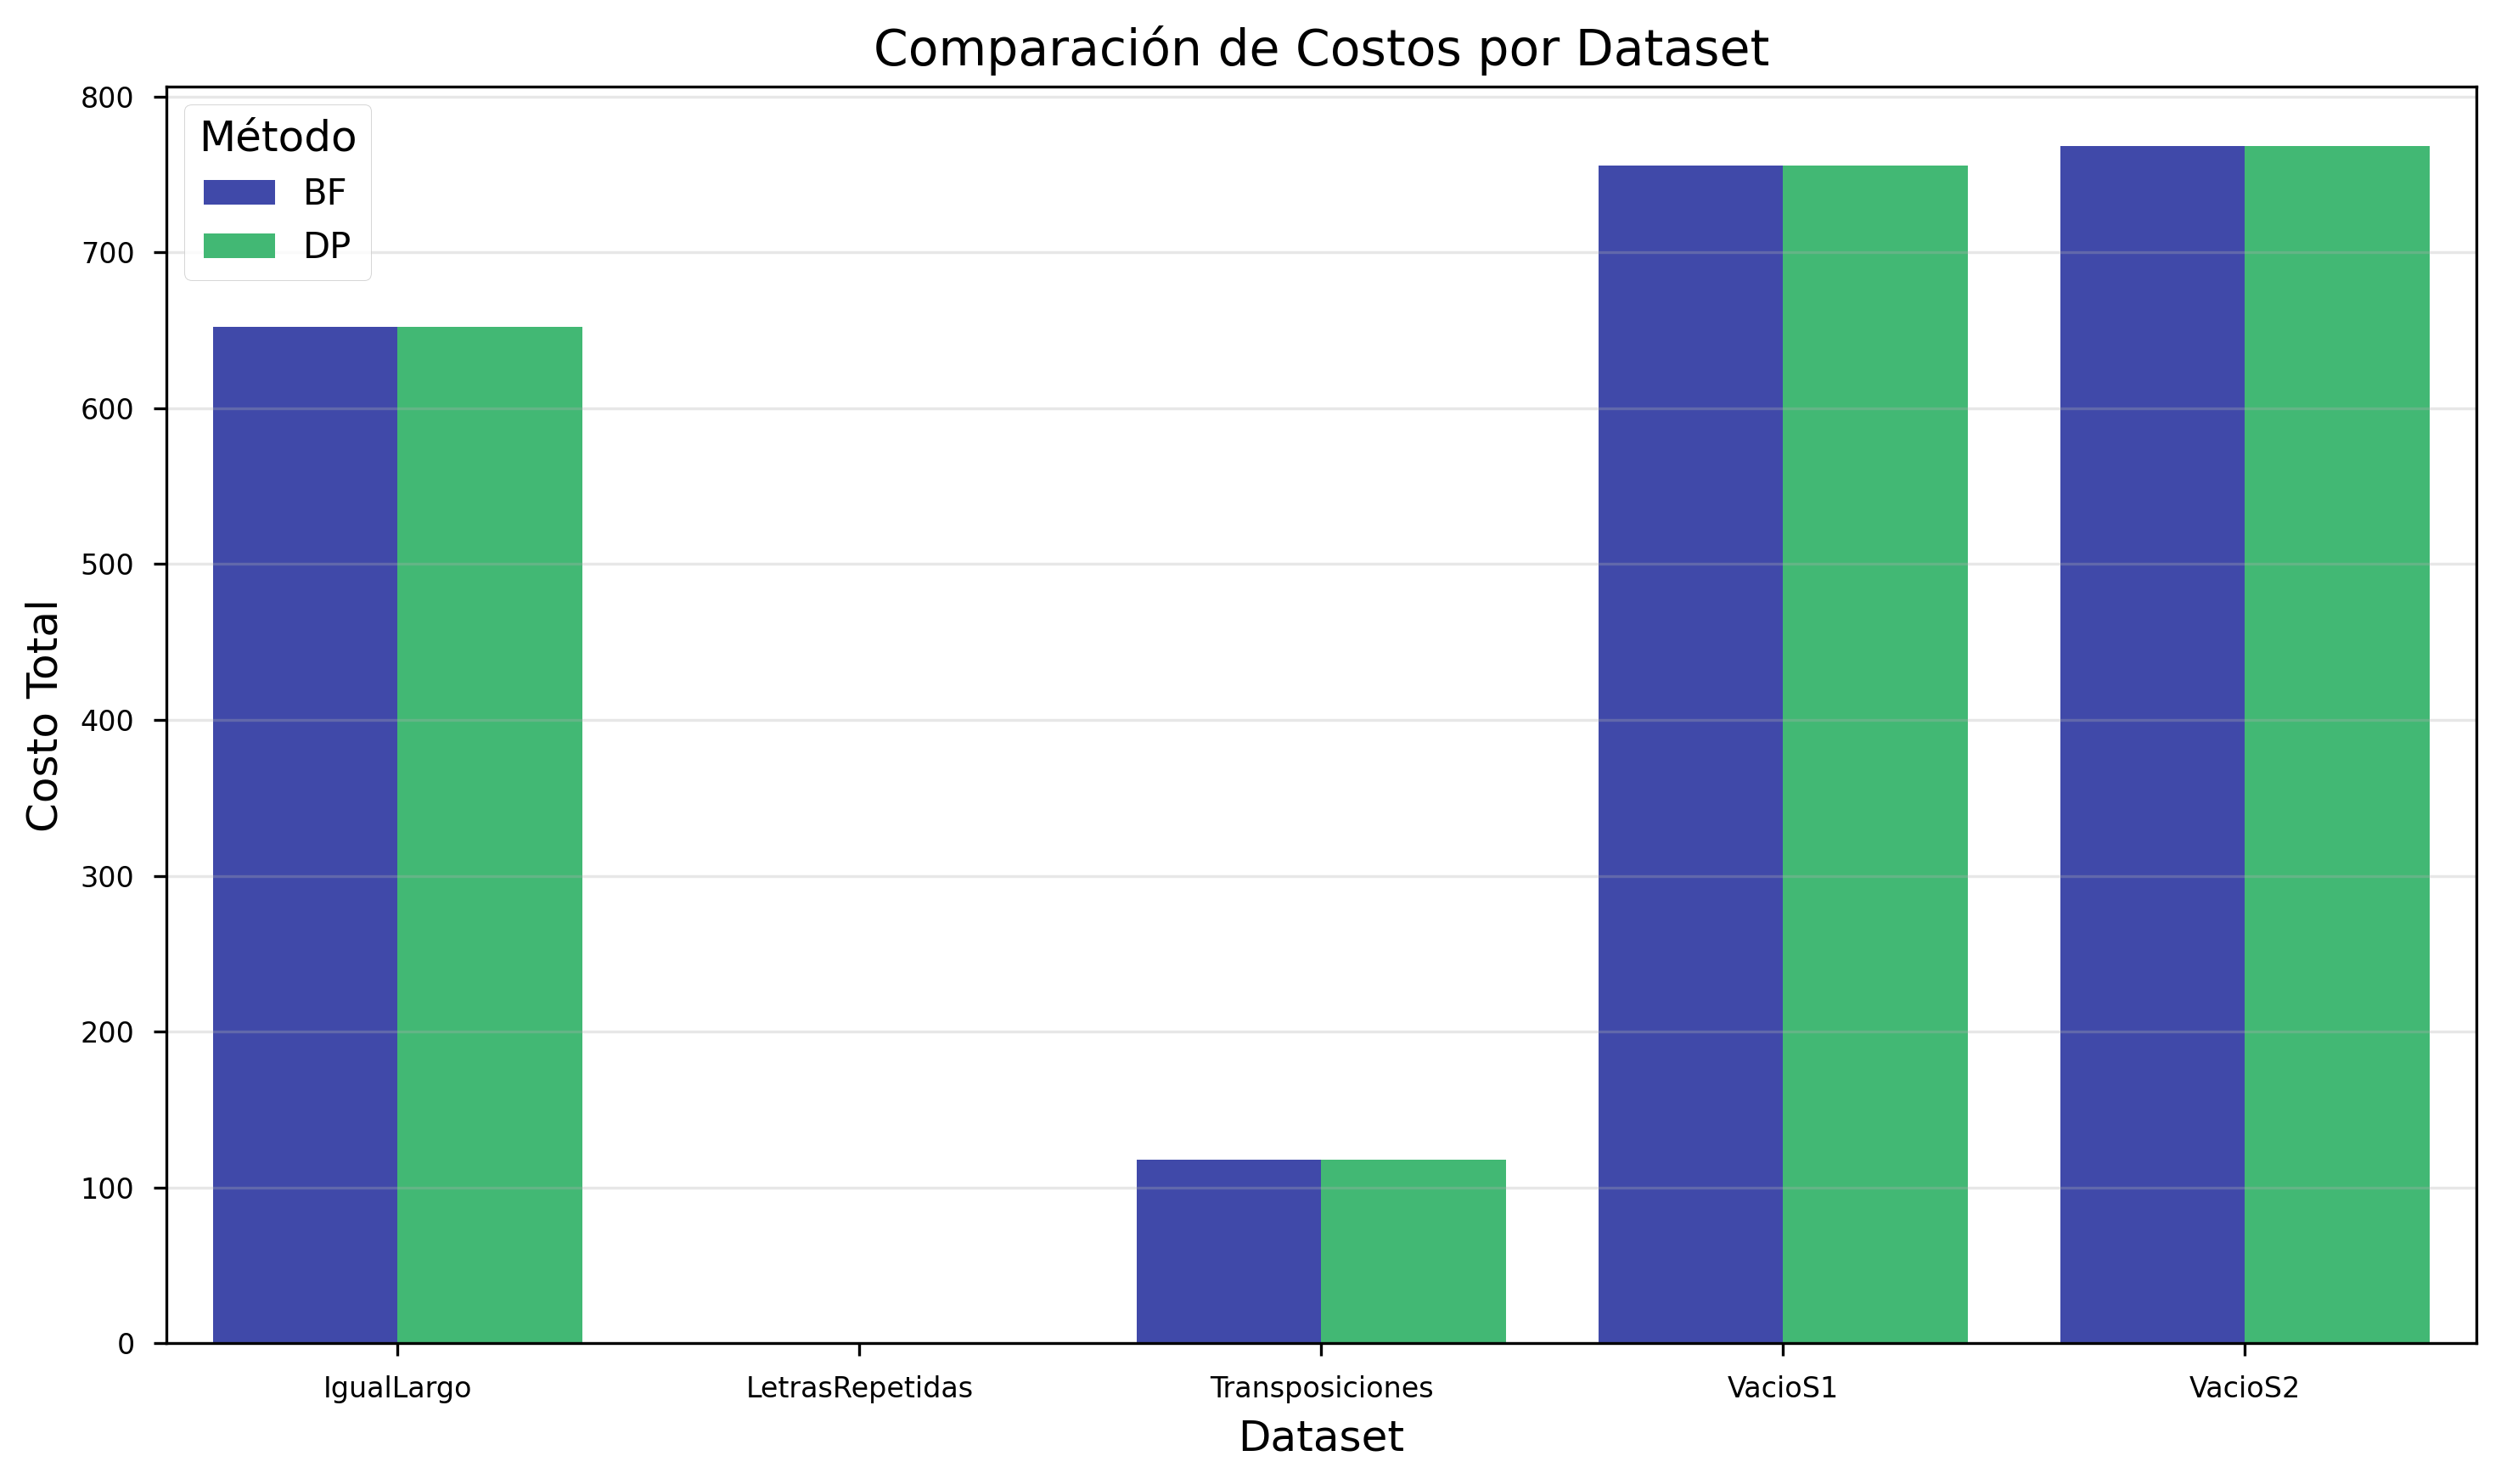
\includegraphics[width=\textwidth]{images/costos_por_dataset.png}
    \end{minipage}%
    \caption{Costos de edicion}
    \label{fig:barplot_1}
\end{figure}
Analizando las figuras 2 y 3 se tiene que las transposiciones juegan un papel relevante puesto que la inclusion de estas aumentan la complejidad, pero esto es por una buena razon,
ya que estas bajan el costo de edicion de las cadenas.

\begin{figure}[H]
    \centering
        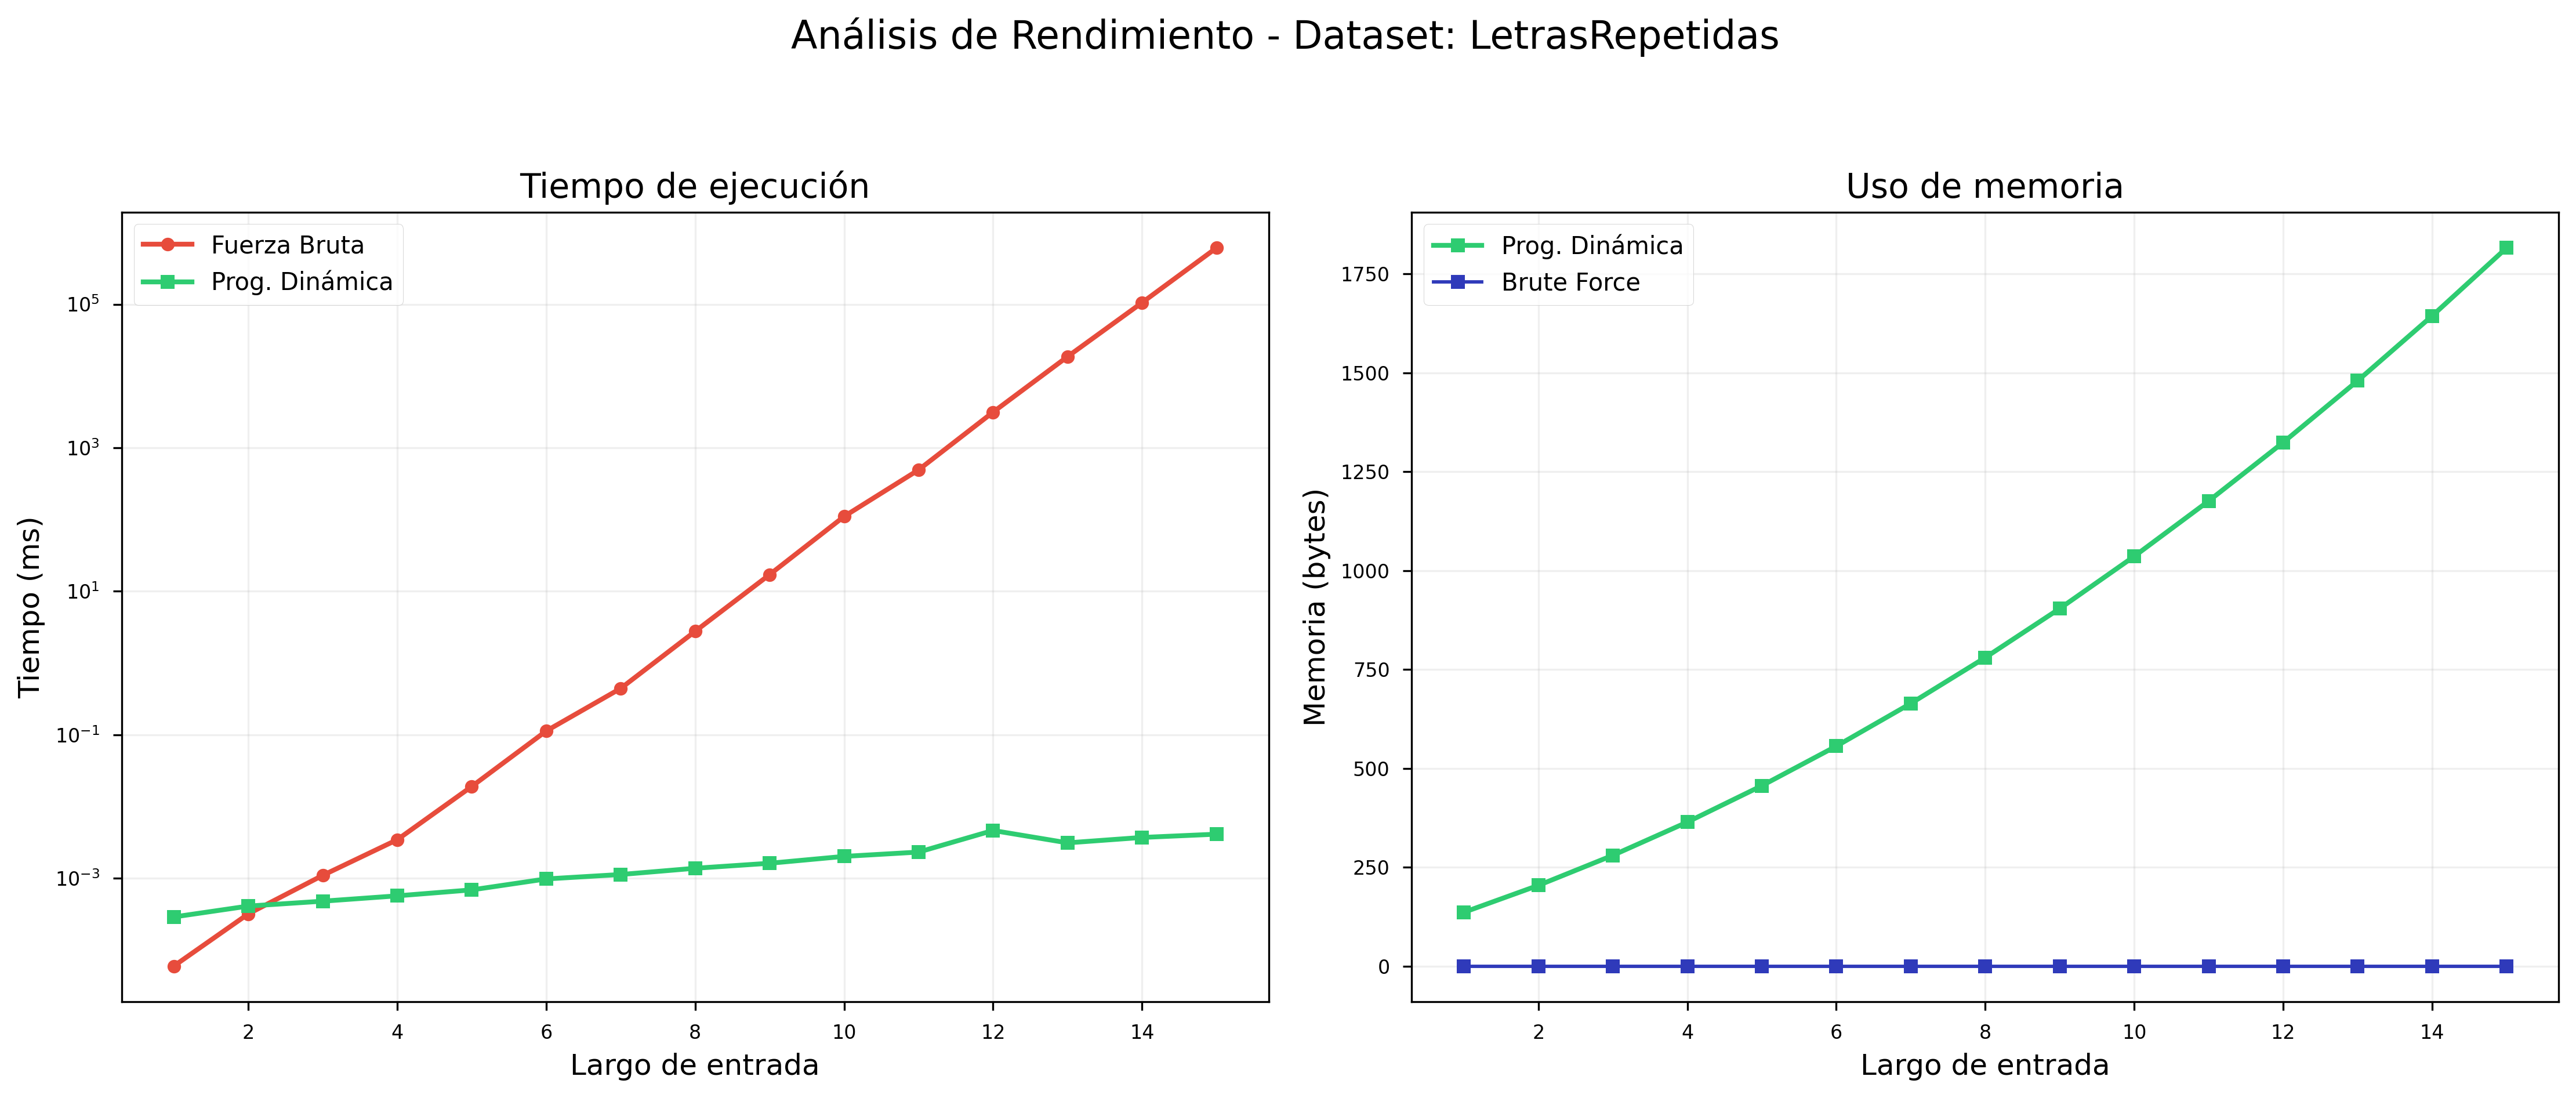
\includegraphics[width=\textwidth]{images/LetrasRepetidas_analisis.png}
    \caption{Cadenas de letras repetidas de largo creciente}
    \label{fig:scatterplot_4}
\end{figure}
Las cadenas repetidas es importante estudiarlas, puesto que estas representan el peor caso en temas de complejidad para fuerza bruta, ya que
las 4 operaciones se realizaran siempre.

\begin{figure}[H]
    \centering
        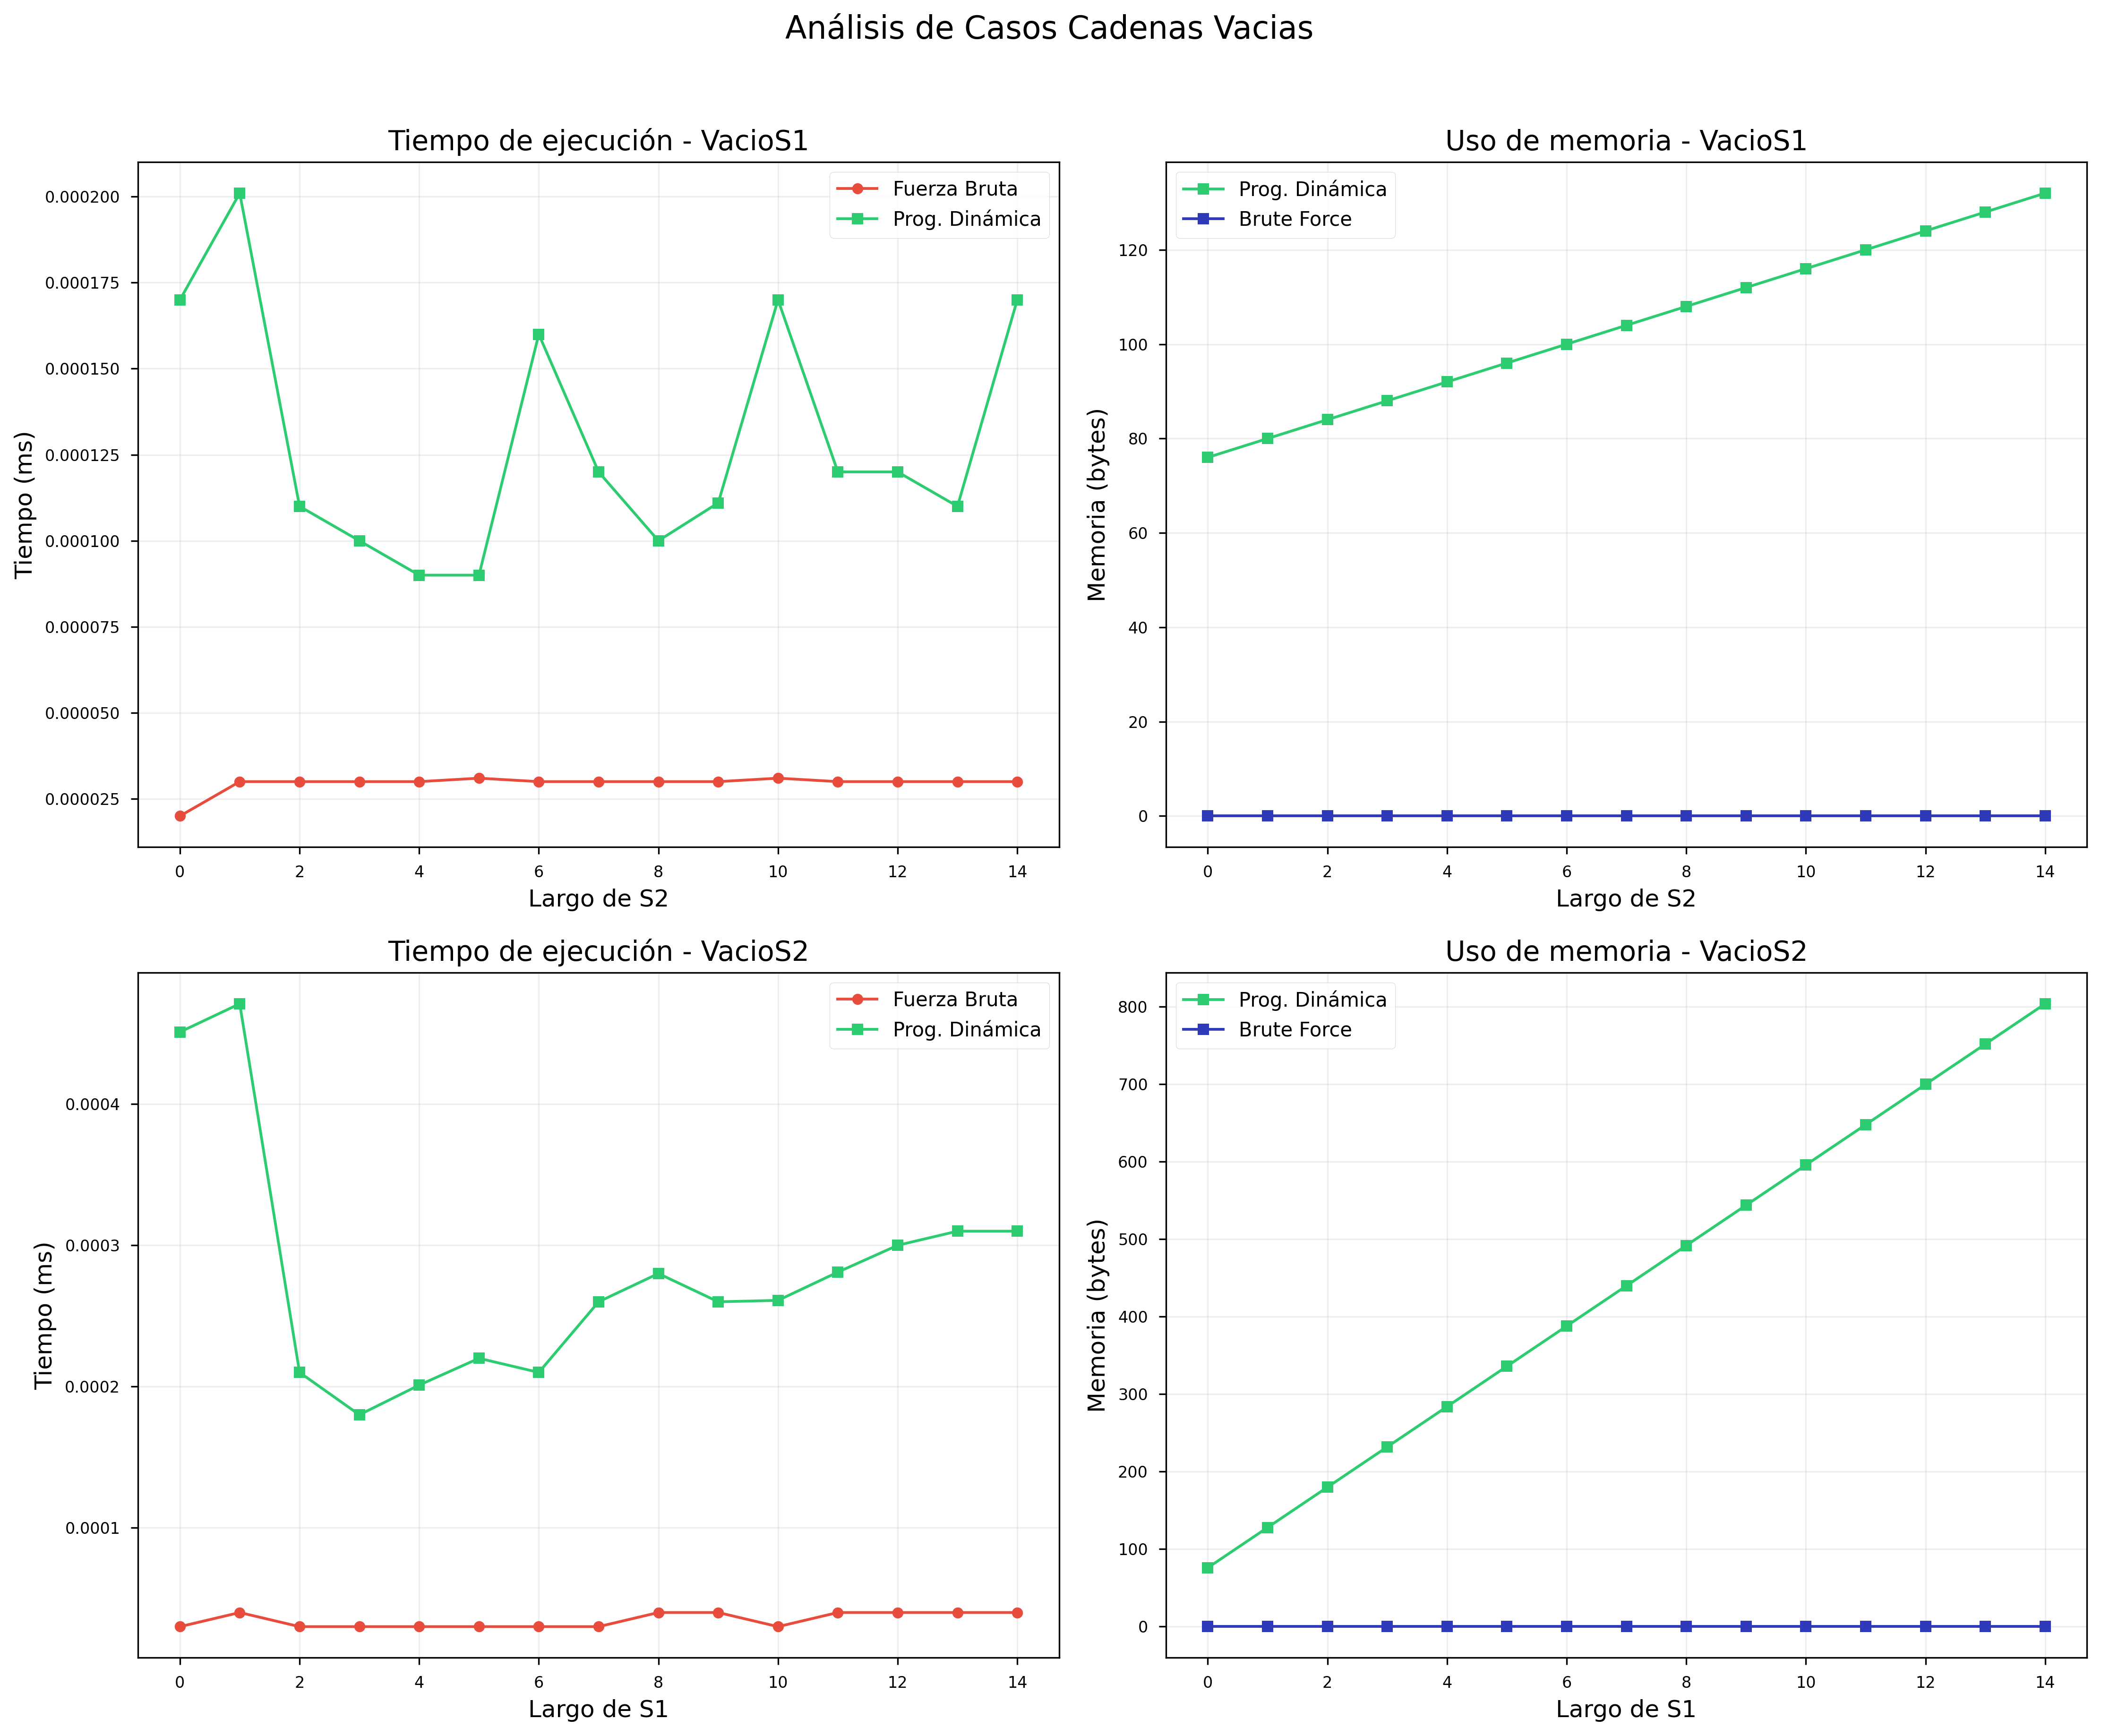
\includegraphics[width=\textwidth]{images/casos_especiales.png} 
        \caption{Casos Cadenas Vacias}
    \label{fig:scatterplot_5}
\end{figure}
Las cadenas vacias representan el mejor caso para fuerza bruta, ya que realiza trabajo lineal en vez de exponencial, por esta misma razon le gana en tiempo de ejecucion
a programacion dinamica.
\begin{figure}[H]
    \centering
        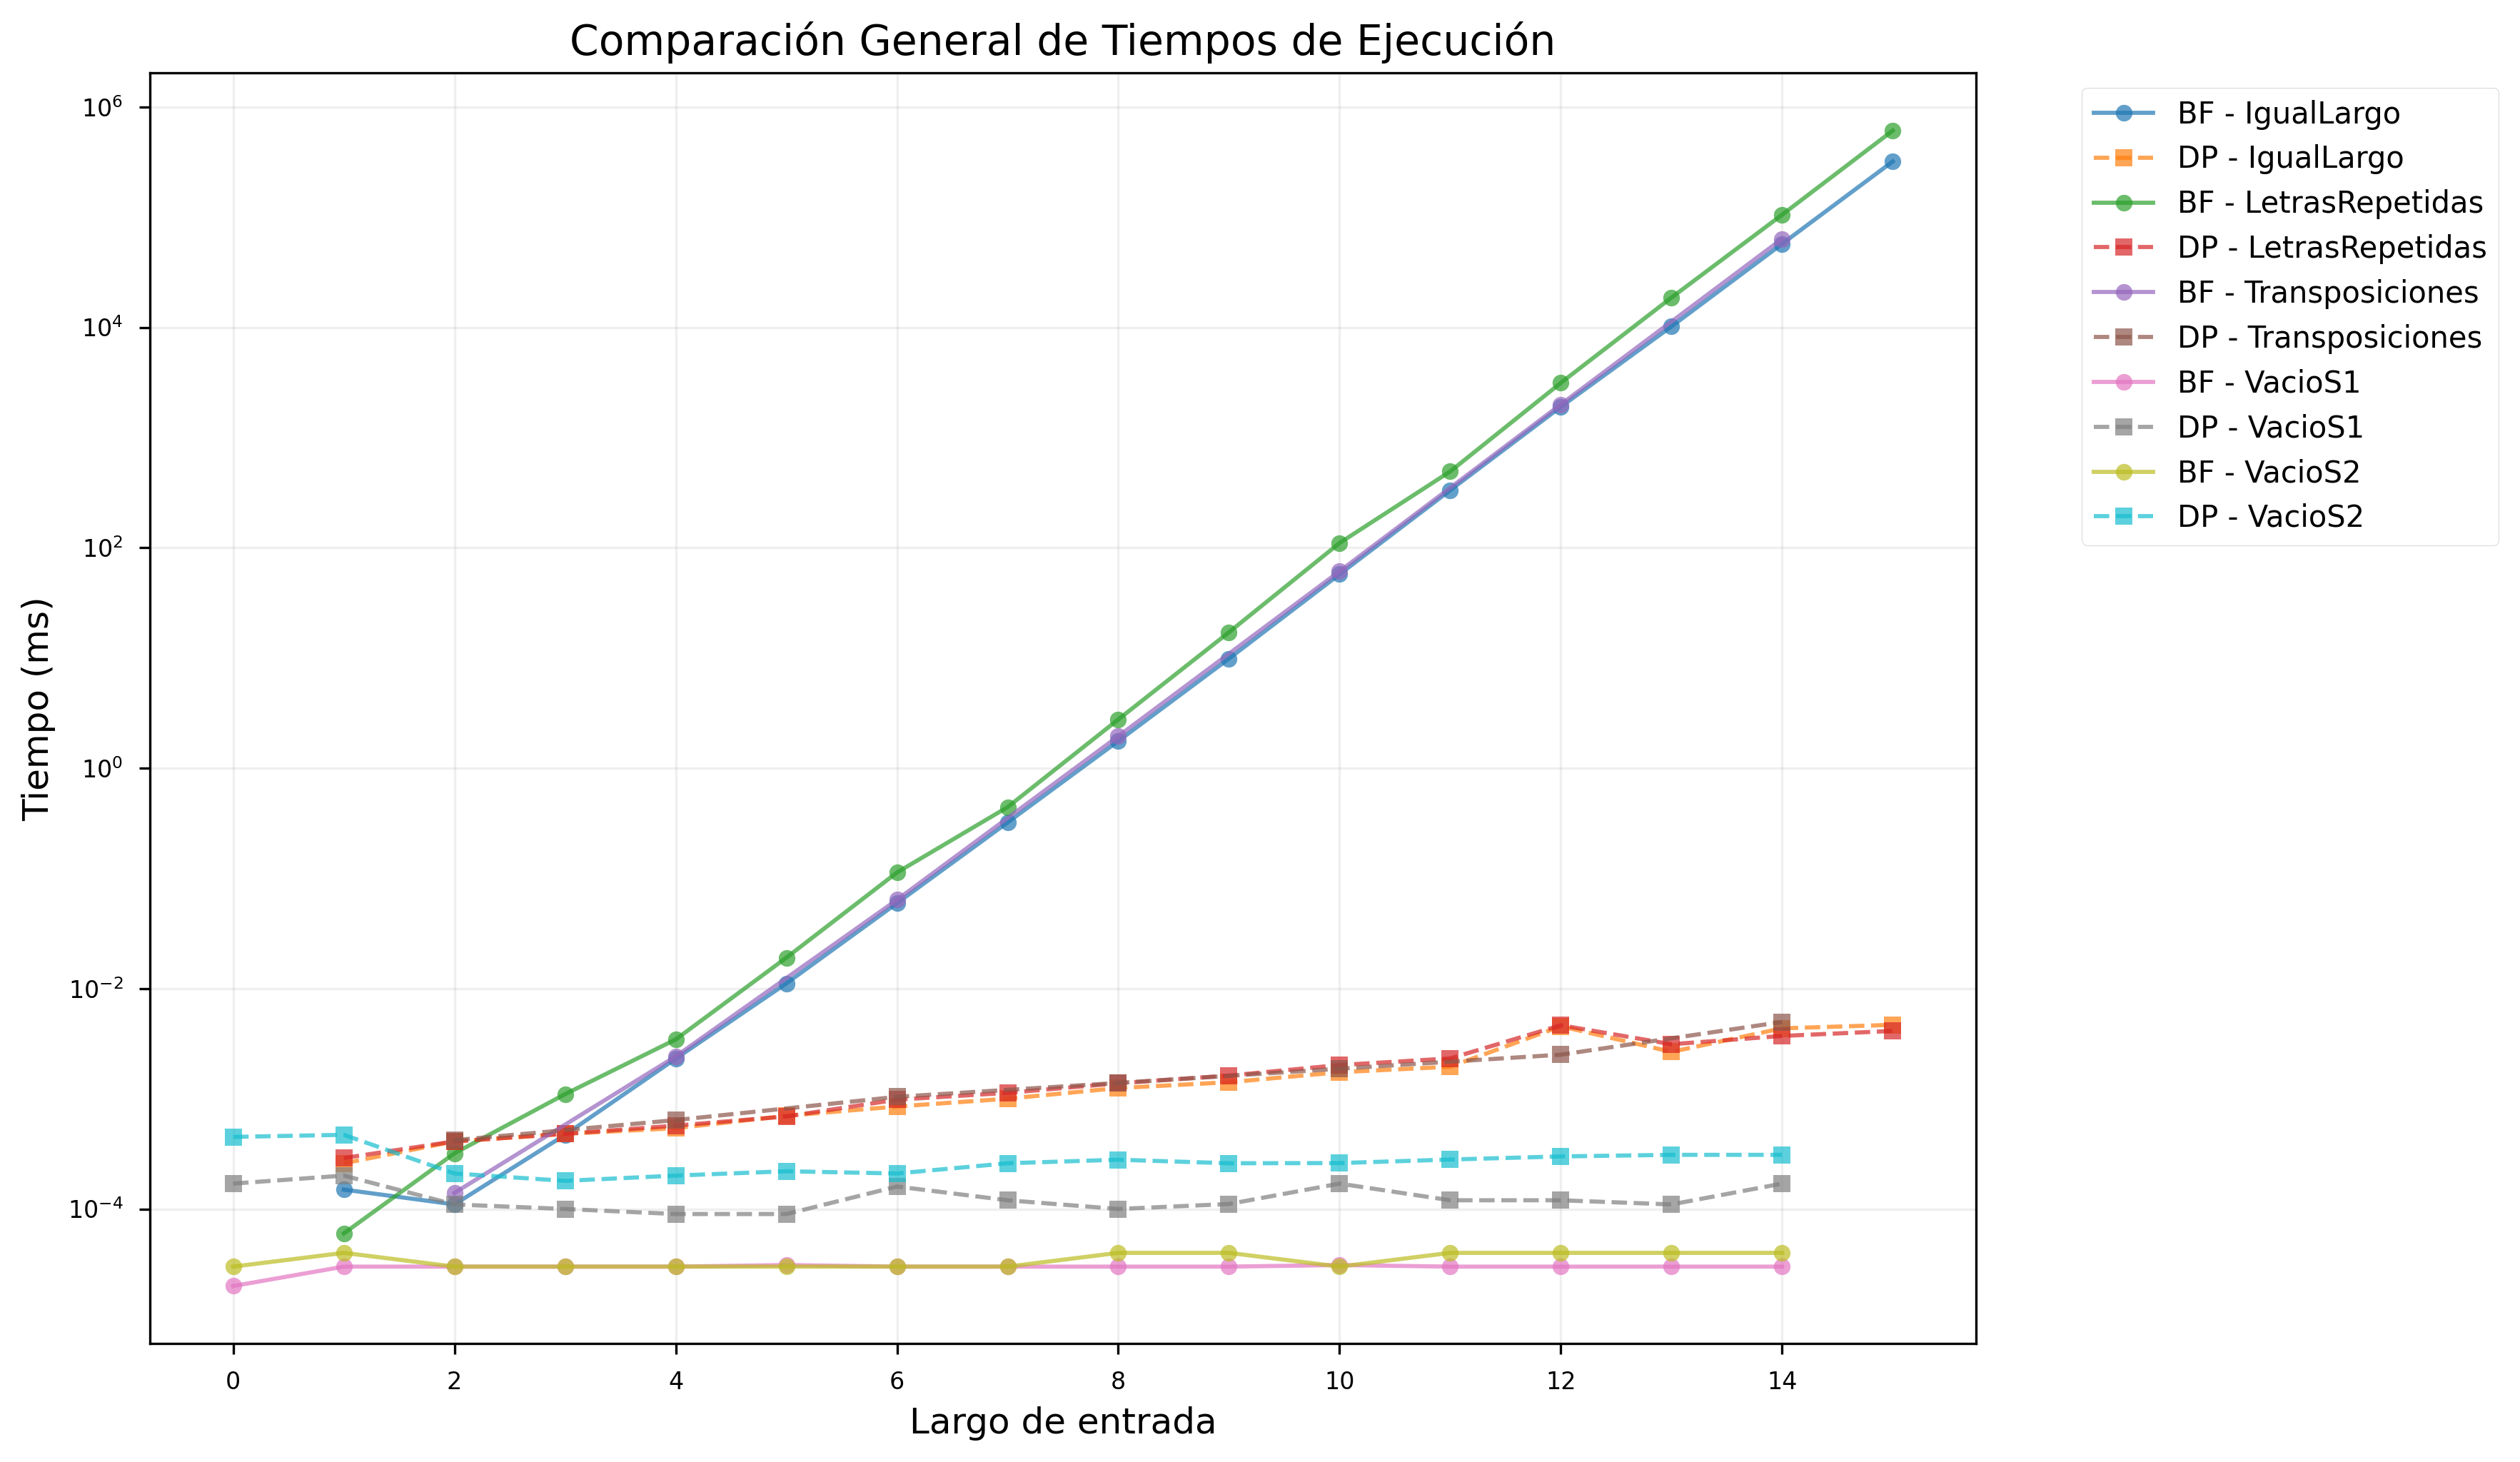
\includegraphics[width=\textwidth]{images/comparacion_general_tiempos.png}    
    \caption{Resumen general de resultados}
    \label{fig:scatterplot_6}
\end{figure}
Finalmente si queremos resolver el problema de la menor distancia, es importante tener en cuenta que el enfoque de fuerza bruta para cadenas vacias 
puede llegar a ser util, sin embargo el enfoque de programacion dinamica es una buena opcion general


\newpage
\section{Conclusiones}
\begin{mdframed}
    \textbf{La extensión máxima para esta sección es de 1 página.}
\end{mdframed}

La conclusión de su informe debe enfocarse en el resultado más importante de su trabajo. No se trata de repetir los puntos ya mencionados en el cuerpo del informe, sino de interpretar sus hallazgos desde un nivel más abstracto. En lugar de describir nuevamente lo que hizo, muestre cómo sus resultados responden a la necesidad planteada en la introducción.

\begin{itemize}
    \item  No vuelva a describir lo que ya explicó en el desarrollo del informe. En cambio, interprete sus resultados a un nivel superior, mostrando su relevancia y significado.
    \item Aunque no debe repetir la introducción, la conclusión debe mostrar hasta qué punto logró abordar el problema o necesidad planteada en el inicio. Reflexione sobre el éxito de su análisis o experimento en relación con los objetivos propuestos.
    \item No es necesario restablecer todo lo que hizo (ya lo ha explicado en las secciones anteriores). En su lugar, centre la conclusión en lo que significan sus resultados y cómo contribuyen al entendimiento del problema o tema abordado.
    \item No deben centrarse en sí mismos o en lo que hicieron durante el trabajo (por ejemplo, evitando frases como "primero hicimos esto, luego esto otro...").
    \item Lo más importante es que no se incluyan conclusiones que no se deriven directamente de los resultados obtenidos. Cada afirmación en la conclusión debe estar respaldada por el análisis o los datos presentados. Se debe evitar extraer conclusiones generales o excesivamente amplias que no puedan justificarse con los experimentos realizados.
\end{itemize}


\newpage

\section{Condiciones de entrega}
% Condiciones generales de tareas de Algoritmos y Complejidad, 20231
  \begin{itemize}
  \item
    La tarea se realizará \tca{individualmente}
    (esto es grupos de una persona),
    sin excepciones.
  \item
    La entrega debe realizarse vía \url{http://aula.usm.cl}
    en un \tca{tarball} en el área designada al efecto,
    en el formato \tca{\texttt{tarea-\tnum-{rol}.tar.gz}}
    (\texttt{rol} con dígito verificador y sin guión).

    Dicho \tca{tarball} debe contener las fuentes en \LaTeXe{}
    (al menos \tca{\texttt{tarea-\tnum.tex}})
    de la parte escrita de su entrega,
    además de un archivo \tca{\texttt{tarea-\tnum.pdf}},
    correspondiente a la compilación de esas fuentes.
  \item Si se utiliza algún código, idea, o contenido extraído de otra fuente, este \textbf{debe} ser citado en el lugar exacto donde se utilice, en lugar de mencionarlo al final del informe. 
  \item
    Asegúrese que todas sus entregas tengan sus datos completos:
    número de la tarea, ramo, semestre, nombre y rol.
    Puede incluirlas como comentarios en sus fuentes \LaTeX{}
    (en \TeX{} comentarios son desde \% hasta el final de la línea)
    o en posibles programas.
    Anótese como autor de los textos.
 
  \item
    Si usa material adicional al discutido en clases,
    detállelo.
    Agregue información suficiente para ubicar ese material
    (en caso de no tratarse de discusiones con compañeros de curso
     u otras personas).
  \item No modifique \texttt{preamble.tex}, \texttt{tarea\_main.tex}, \texttt{condiciones.tex}, estructura de directorios, nombres de archivos, configuración del documento, etc. Sólo agregue texto, imágenes, tablas, código, etc. En el códigos funte de su informe, no agregue paquetes, ni archivos .tex (a excepción de que agregue archivos en \texttt{/tikz}, donde puede agregar archivos .tex con las fuentes de gráficos en \texttt{TikZ}).

\ifprograms
  \item
    Su programa ejecutable debe llamarse \tca{\texttt{tarea\tnum}},
    de haber varias preguntas solicitando programas,
    estos deben llamarse usando el número de la pregunta,
    como \tca{\texttt{tarea\tnum-1}},
    \tca{\texttt{tarea\tnum-2}},
    etc.
    Si hay programas compilados, con en este caso,
    incluya una \tca{\texttt{Makefile}}
    que efectúe las compilaciones correspondientes.

    Los programas se evalúan según que tan claros
    (bien escritos)
    son, si se compilan y ejecutan sin errores o advertencias según corresponda.
    Parte del puntaje es por ejecución correcta con casos de prueba.
    Si el programa no se ciñe a los requerimientos de entrada y salida,
    la nota respectiva es cero.
\fi    
  \item
    %La entrega debe realizarse dentro del plazo indicado en \url{http://aula.usm.cl}:
    La fecha límite de entrega es el día \tca{10 de noviembre de 2024}.

    \begin{center}
        \Large{
          \textbf{NO SE ACEPTARÁN TAREAS FUERA DE PLAZO}.
        }
        \normalsize
    \end{center}
     
    
  \item
    Nos reservamos el derecho de llamar a interrogación
    sobre algunas de las tareas entregadas.
    En tal caso,
    la nota de la tarea será la obtenida en la interrogación.
    \begin{center}
      \Large{
        \textbf{NO PRESENTARSE A UN LLAMADO A INTERROGACIÓN SIN JUSTIFICACIÓN PREVIA SIGNIFICA AUTOMÁTICAMENTE NOTA 0.}
      }
    \end{center}
    
  \end{itemize}

%%% Local Variables:
%%% mode: latex
%%% ispell-local-dictionary: "spanish"
%%% End:

  
% LocalWords:  tarball tar gz pdf min entregable Makefile puntaje
% LocalWords:  Moodle

\newpage
\appendix


\section{Apéndice 1}
\href{https://github.com/MoonTurtlee/T2_3}{Github}


 
\printbibliography

\end{document}


